\section{Define and illustrate the notions of software reuse, reusability and reusable components.}

\textbf{Software reuse} is the reapplication of a variety of kinds of knowledge about one system to another in order to reduce the effort of developing or maintaining that other system. This reused knowledge includes artifacts such as domain knowledge, development experience, requirements, architectural components, design artefacts, code, documentation, and so forth.\newline

\textbf{Reusability} is a general engineering principle whose importance derives from the desire to avoid duplication and to capture commonality in undertaking classes of inherently similar tasks. \newline

\textbf{Software reusability} is the degree to which a software module or other work product can be used in more than one software system.\newline

A \textbf{reusable component} is a software component designed and implemented for the specific purpose of being reused. These reusable components can be requirements, architecture, design, code, test data, and so on.\\


\section{Give two economic and two intellectual justifications for software reuse.}

Two \textbf{economic justifications} for software reuse can be either :
\begin{enumerate}
\item to be \textbf{more productive} by avoiding doing twice the same work,
\item and to have a \textbf{better quality} by reusing already implemented good solutions.\\
\end{enumerate}
Three \textbf{intellectual justifications} for software reuse can be either :
\begin{enumerate}
\item to \textbf{stand on each other's shoulders}, i.e building something new based on previous discoveries or works,
\item  to avoid \textbf{reinventing or reimplement} old stuff,
\item and to focus on what is \textbf{new and relevant}.
\end{enumerate}


\section{Give and explain 3 different software reuse techniques seen throughout the course.}

Here is the list of all software reuse techniques seen throughout the course :
\begin{itemize}
\item Programming abstractions and mechanisms (procedural and data abstraction, data abstraction, encapsulation 
and information hiding, sharing and reuse mechanisms, ...).
\item Design patterns. 
\item Software architecture.
\item Software libraries. 
\item Application frameworks.
\item Software product lines.
\end{itemize}

And here are the explanations on three of them :
\begin{itemize}
\item \textbf{Object-Oriented techniques} : Encapsulation (keeping data and operations that act on this data together), Information Hiding (isolating and hiding design and implementation choices), Code Sharing (capturing and exploiting similarities in data and behavior).\\

\item \textbf{Design patterns} : proposed as a way to reuse extensive architectural experience (expressed as pre-canned architectural fragments). In other words, each pattern describes a problem which occurs over and over again in our environment and then describes the core of the solution to that problem, in such a way that you can use this solution a million times over, without doing it the same way twice.\\

\item \textbf{Frameworks} : implementation techniques used to create families of software applications. A framework represents a common design and partial implementation for the family, i.e a generic solution for a set of similar problems. But, they are incomplete by nature : application-specific functionalities need to be 
filled in by the framework customiser (developer of the application).
\end{itemize}

\section{How and why does object-oriented programming promote modularity and maintainability?}

Object-oriented programming (OOP) promotes modularity and maintainability thanks to its \textbf{abstraction mechanisms}, which are :
\begin{enumerate}
\item \textbf{Encapsulation} : the act of keeping data and operations that act on this data together (objects contain their own data as well as the methods that work on that data).
\item \textbf{Information hiding} : the act of isolating and hiding design and implementation choices (clients of an object only know the set of messages it can receive, and the implementation details of how the messages are processed remain hidden to external clients).
\item \textbf{Polymorphism} : allowing different implementations of a same design to co-exist. This provides a cleaner and more maintainable code (less different method names, less need for conditionals, more implementation freedom, and adds locality to the code)  by delegating responsibilities and implementation choices to the objects .
\item \textbf{Code sharing} : the act of capturing and exploiting similarities in data and behavior (classes enable sharing behaviour among objects, and class hierarchies and inheritance enable reuse of class definitions).
\end{enumerate}
Furthermore, OOP promotes \textbf{maintainability} by viewing programs as collections of loosely connected objects (each object is responsible for specific tasks, the computation proceeds through the interactions of these objects, and all objects can be defined and manipulated in terms of messages).\\
In addition, OOP also promotes the \textbf{development of reusable components} by reducing the interdependency among individual software components (such components can be created and tested as independent units in isolation from the rest of the software system , and these software components permit to treat problems at a higher level of abstraction).


\section{Explain the object-oriented techniques of encapsulation, information hiding, polymorphism
and code sharing and how they relate to software reusability.}

\begin{itemize}
\item  \textbf{Encapsulation} : the act of keeping data and operations that act on this data together (objects contain their own data as well as the methods that work on that data). Encapsulation of both the behaviour and state (grouping the behaviour with the data it acts upon), facilitates modularity, code reuse and maintenance $\rightarrow$ allow to reuse existing objects with all methods and data contained.
\item  \textbf{Information hiding} : the act of isolating and hiding design and implementation choices (clients of an object only know the set of messages it can receive, and the implementation details of how the messages are processed remain hidden to external clients). Doing so restrict the access to objects through a well defined interface : users of an object only know the set of messages it will accept but they do not know how the actions performed in response to a message are carried out (this is the responsibility of the receiving object (through polymorphism) $\rightarrow$ allow to reuse of the defined interface for new objects.
\item  \textbf{Polymorphism} : allowing different implementations of a same design to co-exist. This provides a cleaner and more maintainable code (less different method names, less need for conditionals, more implementation freedom, and adds locality to the code)  by delegating responsibilities and implementation choices to the objects  $\rightarrow$ allow to reuse the same method's name for multiple objects.
\item  \textbf{Code sharing} : the act of capturing and exploiting similarities in data and behavior (classes enable sharing behaviour among objects, and class hierarchies and inheritance enable reuse of class definitions) $\rightarrow$ allow to reuse existing code instead of rewritting it.
\end{itemize}


\section{Explain, using a concrete example, what polymorphism and dynamic binding are, and how
they can help in obtaining more maintainable code.}

\begin{itemize}
\item \textbf{Polymorphism} : as said above, the idea is to allow different implementations of a same design (method, ...) to co-exist. An example could be a same message being sent to objects of different classes :\\
aCircle.\textcolor{red}{surface} and aRectangle.\textcolor{red}{surface} \\
Here, both objects receive the same message, but they can react differently to it, since different classes can provide different implementations for methods with the same name : \\
aCircle $\rightarrow$ surface = $\pi$.$radius^{2}$\\
aRectangle $\rightarrow$ surface = (bottom-top).(right-left)\\
Responsability of how to handle the message is thus decided by the object itself.
\begin{lstlisting}[caption=Pseudocode example of Polymorphism]
Circle {
	Point center; 
	Real radius;
	Real surface() : { 
		pi.radius2
	}
}
Rectangle {
	Real bottom, top, right, left;
	Real surface() : { 
    	(bottom-top)*(right-left) 
    }
}

Real surface (collection) : {
	total = 0
	forall shape in collection: total=total+shape.surface()
	return total
}
\end{lstlisting}
\textbf{Advantages for maintenance} : adding a new shape does not require to change the existing implementation, and no need to know the kind of objects it manipulates as soon as they all share a common interface.

\item \textbf{Dynamic (or late) binding} : when sending a message, the actual receiver of a message is not necessarily known until run-time, thus deferring the mapping of messages to methods until run-time (>< Most traditional languages do this at compile time : static binding).\\
\begin{lstlisting}[caption=Pseudocode example of dynamic binding]
public class DynamicBindingTest {
	public static void main (String args[]) {
    	Vehicule vehicule = new Car();
        vehicule.start();
    }
}

class Vehicule {
	public void Start() {
    	System.out.println("Inside start method of Vehicule - Vroom.");
    }
}

class Car extends Vehicule {
	@Override
    public void start(){
    	System.out.println("Inside start method of Car - Vroom Vroom.");
    }
}

Output : Inside start method of car - Vroom Vroom.
\end{lstlisting}
Here, the method call vehicule.start() is dynamically bound to the overridden Car $\rightarrow$ start() method, because even though vehicule is typed as being of class Vehicule, it is determined at runtime that it contains n object of type Car (and because the method start() is overridden).\\
\textbf{Advantages for maintenance} : adding a new vehicule does not require to change the existing implementation, just create a new class extending Vehicule with a new overridden method start().
\end{itemize}

\section{Explain on a concrete example the concepts of method overriding, self and super calls.}

\begin{itemize}
\item \textbf{Method overriding} : principle that subclasses can re-implement methods that are already implemented in superclasses, allowing a fine-grained reuse (without the client knowing). The resulting overridden method can either overwrite a method with a completely new implementation or can specialise the behaviour of the method defined in its superclass (using the keyword \textcolor{red}{super}).
\begin{lstlisting}[caption=Pseudocode example of Method Overridding]
SomeSuperclass{
	void print: {
		display("Printed in superclass. ")
    }
}
SomeSubclass inherits from SomeSuperclass {
	void print: {
		super.print
        display("Printed in subclass.")
    }
}

test : {
	s = new SomeSubclass()
	s.print
}

After calling test, the program prints:
Printed in superclass. Printed in subclass.
\end{lstlisting}
In this example, the method print in the class SomeSuperclass is overridden by the method in the SomeSubclass. The call using the super keyword specialises the overridden method.

\item \textbf{Self and Super calls} : all methods uses \textcolor{red}{self} calls to reference the receiver object (this keyword in Java, self in Smalltalk) and \textcolor{red}{super} to reference their implementor’s parent.\\
But be carefull ! The key issue in object-oriented programming is that \textbf{self is late/dynamically bound} (method lookup starts again in the class of the receiver object) while \textbf{super is statically bound} (method lookup starts in the superclass of the class of the method containing the super expression, and not in the superclass of the receiver class).

\begin{lstlisting}[caption=Pseudocode example of super calls]
SomeSuperclass{ <---------------------------------- (1)
	void print: {
		display("Printed in superclass. ")
    }
}
SomeSubclass inherits from SomeSuperclass {
	void print: {
		super.print
        display("Printed in subclass.")
    }
}

SubSubclass inherits from SomeSubclass { <--------- (2)
}

test : {
	s = new SubSubclass()
	s.print
}

Here :
(1) super statically refers to this class
(2) SubSubclass is the receiving class
/!\ if super would refer to the super class of the receiver class, we would have a loop !

\end{lstlisting}

\begin{lstlisting}[caption=Pseudocode example of self calls]
SomeSuperclass{ <---------------------------------- (1)
    void printMyself: {
		self.print
	}
    void print: {
		display("Printed in superclass.")
    }
}

SomeSubclass inherits from Some Superclass {
    void print: {
	super.print
	display("Printed in subclass.")
    }
}

SubSubclass inherits from SomeSubclass { <--------- (2)
}

test: {
	s = new SubSubclass()
	s.printMyself
}


Here :
(1) self refers to the receiver
(2) SubSubclass is the receiving class
self will dynamically look up methods starting from this class

\end{lstlisting}
\end{itemize}

\section{How can abstract classes and methods improve reusability?}

First, let's define abstract classes and methods:\\
\begin{itemize}
\item They cannot be instantiated (in Java).
\item But they can provide some method implementations (shared by all subclasses). The methods with a default implementation need to be specialised by subclasses, aswell as methods with a partial implementation.
\item Typically have at least one abstract method, i.e empty implementation that must be provided by 
each subclass.
\end{itemize}

They can improve the reusability by providing "templates" for creating new subclasses that immediately inherits all the implemented methods of the super class. Furthermore, these subclasses can decide whether or not they need to specialise one or more of their inherited methods by overridding them if needed.

\section{Explain, using a concrete example, how a multiple inheritance problem could be modeled
in terms of single inheritance on classes and interfaces in Java.}

Multiple inheritance on classes in Java is not allowed. To achieve the same result in Java, we have to do a little trick. Let’s see with the following example:\\
We have a class \textit{FoodTruck}, which wants to extend the classes \textit{Truck} and \textit{Kitchen}. This will give to our class \textit{FoodTruck} the methods \textit{drive()} and \textit{cook(pizza)} (and their implementation!). However in Java we can’t do that.\\
\begin{center}
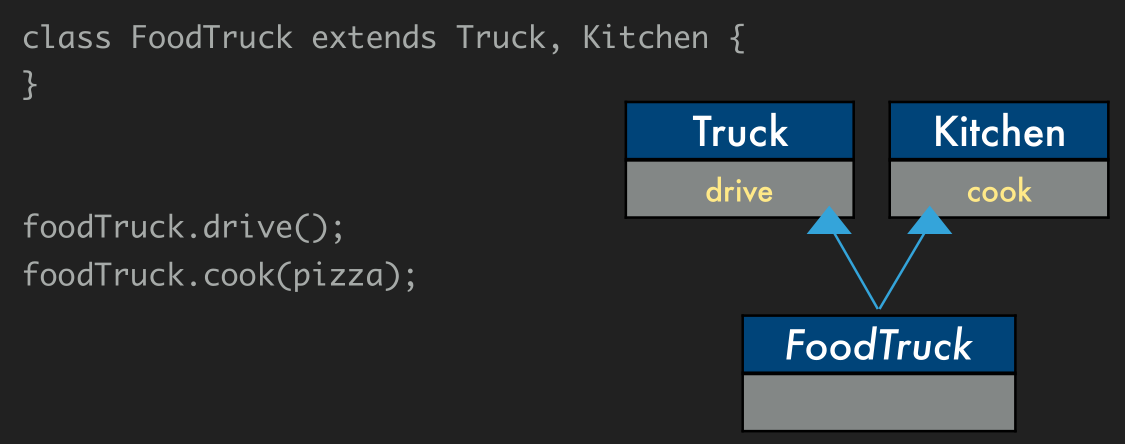
\includegraphics[scale=0.2]{MultipleInheritance_Begin.png}
\end{center}
In order to get both methods, we need to\textbf{ split one of the two classes into an interface and an implementation}. Here, in the following figure, you can see that we split \textit{Kitchen} into the interface \textit{KitchenInterface} and its implementation \textit{Kitchen}. Moreover, \textit{FoodTruck} keeps an instance of the \textit{Kitchen} class. That way, \textit{FoodTruck} has the method \textit{drive()} like before, the method \textit{cook()} with the interface, and the implementation of the latter with the instance of \textit{Kitchen}.\\
\begin{center}
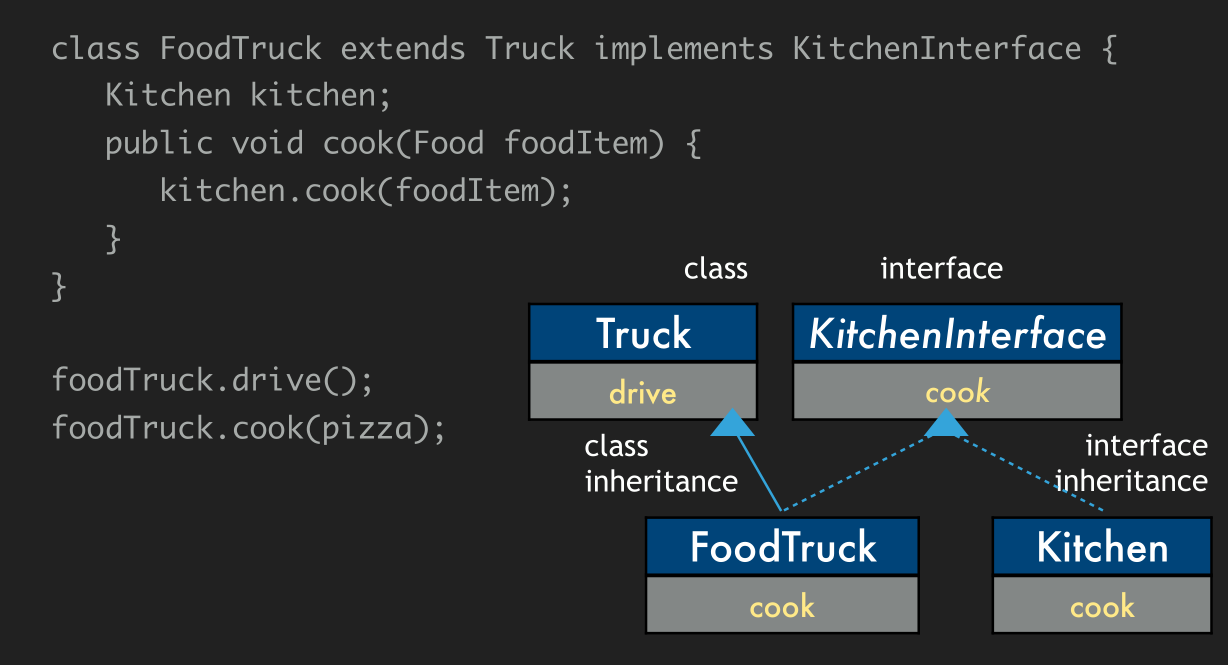
\includegraphics[scale=0.2]{MultipleInheritance_End.png}
\end{center}